% 第 11 题源图的定性重绘：定义域为 0<x<3，零点为 x=1 与开区间端点 x=3。
% 曲线形态与端点来自固定 PDF 第 1 页；坐标比例为示意，不作为函数条件。
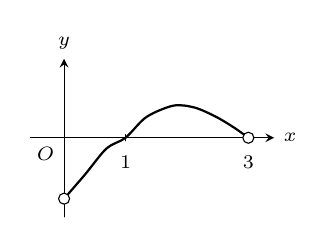
\begin{tikzpicture}[x=.78cm,y=.85cm,>=stealth,line cap=round,line join=round,
  every node/.style={font=\scriptsize}]
  \draw[->] (-.55,0)--(3.42,0) node[right] {$x$};
  \draw[->] (0,-1.18)--(0,1.18) node[above] {$y$};
  \node[below left] at (0,0) {$O$};
  \draw (.0,.045)--(.0,-.045);
  \draw (1,.045)--(1,-.045) node[below=2pt] {$1$};
  \draw (3,.045)--(3,-.045) node[below=2pt] {$3$};
  \draw[thick] plot[smooth] coordinates {
    (0,-.91) (.34,-.55) (.69,-.16) (1,0) (1.34,.31)
    (1.78,.48) (2.13,.45) (2.48,.31) (2.77,.15) (3,0)
  };
  \filldraw[fill=white] (0,-.91) circle[radius=2pt];
  \filldraw[fill=white] (3,0) circle[radius=2pt];
\end{tikzpicture}
